\subsection{Neighbour pitch mutation}
This mutation is can be seen as an optimization. Wrong intervals introduced in \ref{sec:rater:neighbourpitch} are being selected for mutation. Out of this selection of intervals, one is randomly chosen for mutation. In order to fix the chosen interval, a note or a chord needs to be transposed. An interval consists of a start note and an end note. For a chord, only the root note is considered for the interval, but the whole chord is transposed if selected. Consider the following notes:
$P$ is previous note before the middle interval, $S$ is the start note of middle interval, $E$ is the end note of middle interval and $N$ is the next note after the middle interval. These four elements create the three following intervals: $PS$ the previous interval, $SE$ the middle interval and the $EN$ next interval. Every interval has a step size called the semitone: the previous semitone, the middle semitone and the next semitone. 
\\
This mutation selects the end note $E$ or the start note $S$ for mutation. There are four cases. The first case is when the absolute value of the next semitone is higher than the previous semitone and the direction of the middle interval is different from the next interval. The direction is the sign of the semitone. This is illustrated at figure \ref{fig:npmut_case1}. Here, the end note $E$ will be transposed upwards.

\begin{figure}[H]
	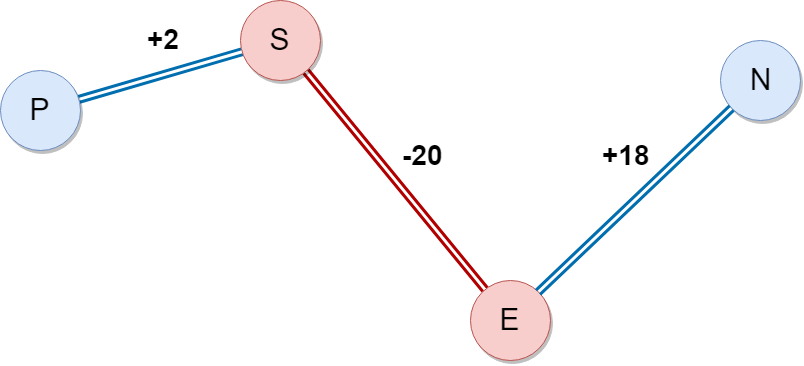
\includegraphics[width=\linewidth]{Fotos/np_mutation/Case1.png}
	\caption{Case where note E is going to be transposed upwards.}
	\label{fig:npmut_case1}
\end{figure}

The next case is illustrated at figure \ref{fig:npmut_case2}. The absolute value of the next semitone is higher than the previous one just like the previous case, but the direction of the middle interval, however, is not different from the next interval. Here, the start note $S$ will be transposed downwards.

\begin{figure}[H]
	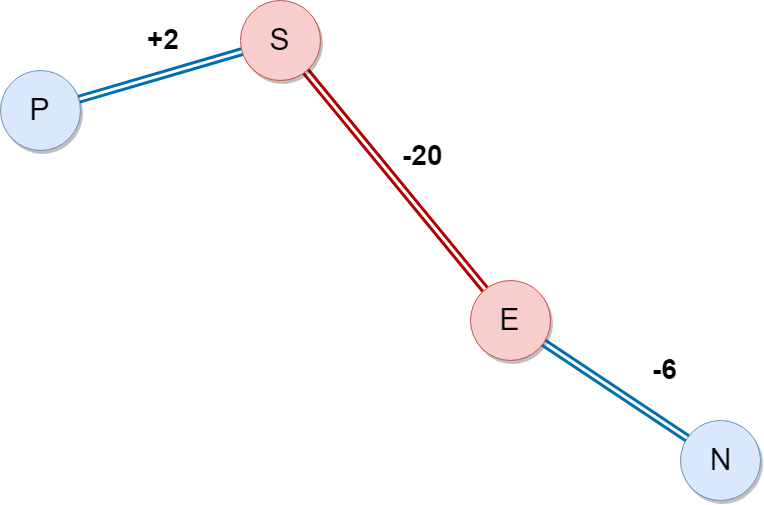
\includegraphics[width=\linewidth]{Fotos/np_mutation/Case2.png}
	\caption{Case where note S is going to be transposed downwards.}
	\label{fig:npmut_case2}
\end{figure}

There are two cases left, they both have similar behavior but in an opposing way. Here, the absolute value of the next semitone is lower than the previous unlike the previous cases. Now the previous interval direction is compared with the middle interval direction. If the direction of the middle interval and previous interval are the same the end note $E$ is selected, else the start note $S$. In all these cases, if the start note is selected, it will be transposed in the direction of the middle interval. If the end note is selected, it will be transposed in the opposite direction of the middle interval. The note will be transposed according to the scale the song tend to follow.